%%%%%%%%%%%%%%%%
\section{Tuesday 11 September:  Color Models}
%%%%%%%%%%%%%%%%

\subsection{Anti-Aliasing}

Oblique lines of the same length have less color intensity because the pixels are more scattered.  

Anti-aliasing can be fixed with greyscale.

Grey level intensity proportional to the area covered.  

Randomizing subpixels (Sampling error)

\subsection{Character Generation}

Bitmap fonts v/s outline fonts

Ideal:  Start with outline fonts, render into font cache.  

\subsection{Color Models}

Parts of a color model:

\begin{itemize}
	\item Hue.  Distinguishes b/n colors, relates to ``dominant wavelength''
	\item Saturation.  How far a color is from grey.  ``Excitation purity.''
	\item Light.  Perceived intensity, reflected.  ``Luminescence.''
\end{itemize}

Humans are less sensitive to variations in blue than variations in red or green.  

\subsubsection{RGB:  ``Emitting Light''}

RGB is device-oriented.  

\

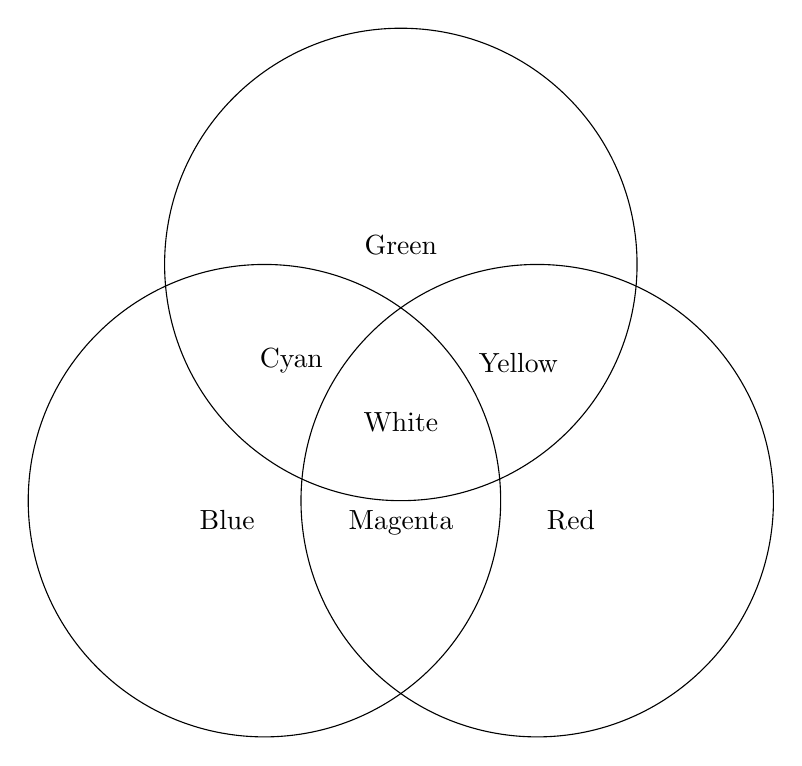
\begin{tikzpicture}[x=20mm,y=20mm]
	\coordinate (G) at ({cos(90)},{sin(90)});
	\coordinate (B) at ({cos(210)},{sin(210)});
	\coordinate (R) at ({cos(330)},{sin(330)});
	\coordinate (C) at ({0.5*cos(150)},{0.5*sin(150)});
	\coordinate (M) at ({0.5*cos(270)},{0.5*sin(270)});
	\coordinate (Y) at ({0.5*cos(30)},{0.5*sin(30)});
	\draw (G) circle (1.5);
	\draw (B) circle (1.5);
	\draw (R) circle (1.5);
	\path (G) node [above] {Green};
	\path (B) node [below left] {Blue};
	\path (R) node [below right] {Red};
	\path (C) node [above left] {Cyan};
	\path (M) node [below] {Magenta};
	\path (Y) node [above right] {Yellow};
	\path (0,0) node [] {White};
\end{tikzpicture}

There is no wavelength that gives ``magenta.'' we perceive it as the mixture of two colors.  

\subsubsection{RGB Cube}

\tdplotsetmaincoords{70}{110}
\begin{tikzpicture}[scale=5,tdplot_main_coords]

%set up some coordinates 
%-----------------------
\coordinate (O) at (0,0,0);
\coordinate (R) at (0,0,1);
\coordinate (G) at (0,1,0);
\coordinate (B) at (1,0,0);
\coordinate (M) at (1,0,1);
\coordinate (C) at (1,1,0);
\coordinate (Y) at (0,1,1);
\coordinate (W) at (1,1,1);

\draw[thick,->] (O) -- ($1.2*(B)$) node[anchor=north east]{B};
\draw[thick,->] (O) -- ($1.2*(G)$) node[anchor=north west]{G};
\draw[thick,->] (O) -- ($1.2*(R)$) node[anchor=south]{R};

\draw (R) -- (M) -- (B) -- (C) -- (G) -- (Y) -- (R);
\draw (C) -- (W);
\draw (M) -- (W);
\draw (Y) -- (W);

\path (O) node [above right] {Black};
\path (W) node [below left] {White};
\path (C) node [below] {Cyan};
\path (M) node [left] {Magenta};
\path (Y) node [right] {Yellow};



%\foreach \i in {0, 30, 60, ..., 360}{
%	\foreach \j in {0, 0.2, 0.4,...,1}{
%		\draw (\j, {cos(\i)*0.2},{sin(\i)*.2)}) -- (\j, {cos(\i+30)*0.2},{sin(\i+30)*.2)}); 
%	}
%}

\end{tikzpicture}


\subsubsection{CMY:  ``Absorbing Light.''}

Printers use CMY (Cyan, Magenta, Yellow)

$$
\left[
	\begin{array}{c}
		\text{C} \cr
		\text{M} \cr
		\text{Y} \cr
	\end{array}
\right]
=
\left[
	\begin{array}{c}
		\text{1} \cr
		\text{1} \cr
		\text{1} \cr
	\end{array}
\right]
-
\left[
	\begin{array}{c}
		\text{R} \cr
		\text{G} \cr
		\text{B} \cr
	\end{array}
\right]
$$

\subsubsection{HSV Model}

Hue, Saturation, Value

Cone shaped

More artist-oriented.  

\subsection{Modeling the World}

Surface modeling, Materials properties, Scene graph organization

Surface representation techniques:  

\qquad Polygon meshes

\qquad Triangle meshes (in this class)

Polygon rendering:

\qquad Consider each polygon

\qquad Project onto a 2D viewing screen.  


